%%%%%%%%%%%%%%%%%%%%%%%%%%%%%%%%%%%%%%%%%%%%%%%%%%%%%%%%%%%%%%%%%%%%%%%%%%%%%%%%%%
\begin{frame}[fragile]\frametitle{}
\begin{center}
{\Large Pranayam प्राणायाम}
\end{center}
\end{frame}

%%%%%%%%%%%%%%%%%%%%%%%%%%%%%%%%%%%%%%%%%%%%%%%%%%%%%%%%%%%
\begin{frame}[fragile]\frametitle{Introduction}

Tasmin sati shwasa pravasa-yorgati vicchedaha Pranayamah

तस्मिन् सति श्वासप्रश्वाससयोर्गतिविच्छेद:||

	\begin{itemize}
	\item Pranayama  helps  in  retraining 
and  regulating  breath. 
Rhythmic  breathing  calms 
down  the  mind.  
	\item Swami 
Vivekananada  explained  this 
trough  a  story  in  which  a 
minister  made  his  escape  and 
descended forms the tower by 
means  of  a  rope  and  silken 
thread,  tied  to  a  beetle  with 
honey to its feelers 
	\end{itemize}

\end{frame}

%%%%%%%%%%%%%%%%%%%%%%%%%%%%%%%%%%%%%%%%%%%%%%%%%%%%%%%%%%%
\begin{frame}[fragile]\frametitle{Why Talk about Breath? }


	\begin{itemize}
	\item   Emotions control breathing ‐ breathing can control  g g
emotions
	\item    Only physiological process both voluntary and 
involuntary involuntary
	\item   Physical body and mind need ''energy'' for functioning
	\item    Energy and matter are inter convertible
	\item   Prana is the link between mind and body
	\item   Voluntary changes in breathing can bring about change 
in energy patterns in energy patterns
	\item   Cosmic inhalation and exhalation creation and 
dissolution
	\item   Involuntary breath controlled by primitive parts of the 
brain
	\end{itemize}

\tiny{(Ref: Eight Limbs of Yoga - Subhash Mittal)}

\end{frame}

%%%%%%%%%%%%%%%%%%%%%%%%%%%%%%%%%%%%%%%%%%%%%%%%%%%%%%%%%%%
\begin{frame}[fragile]\frametitle{What is Pranayama?}


	\begin{itemize}
	\item  Fourth of the eight limbs of yoga g y g
	\item  Compound word – ``prana'' + ``ayama''
	\item  Prana = pra (prefix) + an (to breathe, to live)
	\item  ``prana'' is life‐force, the cosmic vital energy
	\item  ``ayama'' means to stretch, expand, control
	\item  Pranayama is to expand and control prana
	\item  Breath is a gross manifestation of prana, usually 
equated with prana equated with prana
	\item  Breathing techniques help control prana in 
different ways
	\end{itemize}

\tiny{(Ref: Eight Limbs of Yoga - Subhash Mittal)}

\end{frame}

%%%%%%%%%%%%%%%%%%%%%%%%%%%%%%%%%%%%%%%%%%%%%%%%%%%%%%%%%%%
\begin{frame}[fragile]\frametitle{Five Sheaths (Koshas) }


	\begin{itemize}
	\item  Annamaya Kosha: physical sheath sustained 
by food (anna)
	\item Pranamaya kosha: Vital sheath sustained by 
breath (prana)
	\item Manomaya kosha: Mental sheath  cognition, 
willing, desires etc
	\item Vijnanamaya kosha: intellectual and intuitive 
sheath
	\item Anandamaya kosha: Bliss sheath
	\end{itemize}

\tiny{(Ref: Eight Limbs of Yoga - Subhash Mittal)}

\end{frame}

%%%%%%%%%%%%%%%%%%%%%%%%%%%%%%%%%%%%%%%%%%%%%%%%%%%%%%%%%%%
\begin{frame}[fragile]\frametitle{Five Pranas }


	\begin{itemize}
	\item  Prana: head to navel; all intakes - food, water, air, 
sensory impressions
	\item Apana: navel to root chakra;  Elimination (stool, urine, 
all fluids CO2) reproduction; also negative feelings all fluids, CO2), reproduction; also negative feelings 
and emotions; basis for all immune functions
	\item Udana: navel to head; growth of body, speech, 
enthusiasm and will enthusiasm and will
	\item  Samana: periphery to navel; digestion, absorbing O2, 
homogenize mental impressions
	\item  Vyana: navel to periphery; all circulations - nutrients; 
helps all other pranas
	\end{itemize}

\tiny{(Ref: Eight Limbs of Yoga - Subhash Mittal)}

\end{frame}

%%%%%%%%%%%%%%%%%%%%%%%%%%%%%%%%%%%%%%%%%%%%%%%%%%%%%%%%%%%
\begin{frame}[fragile]\frametitle{Five Up Pranas }


	\begin{itemize}
	\item  Naga: burping, throwing, stretching, 
salivation, hiccups
	\item  Kurma: movement of the eyelids and size of 
iris to control intensity of light
	\item  Krikara: sneezing, coughing, reactions to pain, 
hunger, thirst
	\item  Devdatta: yawning, sleep
	\item  Dhananjaya: produce phlegm, provides 
nourishment, inflates the body after death nourishment, inflates the body after death
	\end{itemize}

\tiny{(Ref: Eight Limbs of Yoga - Subhash Mittal)}

\end{frame}

%%%%%%%%%%%%%%%%%%%%%%%%%%%%%%%%%%%%%%%%%%%%%%%%%%%%%%%%%%%
\begin{frame}[fragile]\frametitle{Physiology of Breathing }

   \begin{columns}
    \begin{column}[t]{0.4\linewidth}
	
\begin{center}
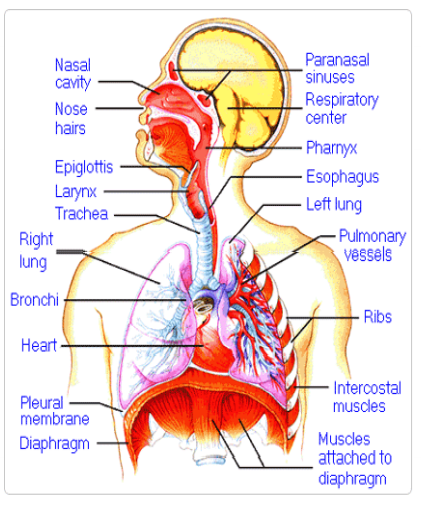
\includegraphics[width=0.9\linewidth,keepaspectratio]{images/yog38}
\end{center}


    \end{column}
    \begin{column}[t]{0.6\linewidth}
	\begin{itemize}
	\item  Nose, windpipe, lungs, circulatory system and associated muscles transport O2
	\item  Blood density higher at lower part of the lungs
	\item   Shallow breathing inefficient in carrying O2 in blood cells to carrying O2 in blood to cells
	\item   Hemoglobin carries O2 to cells 
and CO2 back from the cell to the heart 
	\item  Gas exchange (O2 - CO2) - respiration - happens at the 
cell level
	\end{itemize}

    \end{column}
  \end{columns}

\tiny{(Ref: Eight Limbs of Yoga - Subhash Mittal)}

\end{frame}

%%%%%%%%%%%%%%%%%%%%%%%%%%%%%%%%%%%%%%%%%%%%%%%%%%%%%%%%%%%
\begin{frame}[fragile]\frametitle{Components of Breathing}


	\begin{itemize}
	\item  Inhalation purak पूरक
	\item  Exhalation rechak रेचक
	\item Breath Retention kumbhak कुम्भक
	\begin{itemize}
	
	\item External retention bahirkumbhak बहिर्कुम्भक
	\item Internal retention antarkumbhak अन्तर्कुम्भक
	\end{itemize}
	
	\end{itemize}

\tiny{(Ref: Eight Limbs of Yoga - Subhash Mittal)}

\end{frame}

%%%%%%%%%%%%%%%%%%%%%%%%%%%%%%%%%%%%%%%%%%%%%%%%%%%%%%%%%%%
\begin{frame}[fragile]\frametitle{Breathing Habits}


	\begin{itemize}
	\item  Shallow breathing is most common  g
	\item  A sob of grief, anger, anxiety etc. can dramatically 
effect breathing
	\item   Anxiety associated with shallow chest breathing • Anxiety associated with shallow chest breathing
	\item  Unfortunately, tummy tucked in is fashionable
	\item   Autonomic nervous system - sympathetic and  parasympathetic
	\item  Under ''fight or flight'' - sympathetic takes over - chest 
breathing breathing
	\item   Holding breath beyond capacity prevented by ANS 
regulation
	
	\end{itemize}

\tiny{(Ref: Eight Limbs of Yoga - Subhash Mittal)}

\end{frame}



%%%%%%%%%%%%%%%%%%%%%%%%%%%%%%%%%%%%%%%%%%%%%%%%%%%%%%%%%%%
\begin{frame}[fragile]\frametitle{Pranayama in Practice}


	\begin{itemize}
	\item  Ujjayi breathing
	\item  Sectional deep breathing
	\begin{itemize}
	
	\item  Clavicle (upper part of lungs)
	\item Thoracic (middle part of lungs)
	\item Diaphragmatic (lower part of lungs)
	\item  Full 3-part (yogic) breathing	
	\end{itemize}
	\item Kapalabhati (breath of fire)
	\item Bhramari (bumble bee breath)
	\item Anulom Vilom, Nadi shuddhi (alternate nostril 
breathing)
	\end{itemize}

\tiny{(Ref: Eight Limbs of Yoga - Subhash Mittal)}

\end{frame}